\documentclass[]{article}

\usepackage[utf8]{inputenc}
\usepackage{amsmath}
\usepackage{amssymb}
\usepackage{amsthm}
\usepackage{amsfonts}
\usepackage{graphicx}
\usepackage{capt-of}
\usepackage{listings}
\usepackage{siunitx}
\usepackage[section]{placeins}
\usepackage{float}



% Oppgavenummerering %
\renewcommand\thesection{Task \arabic{section}}
\renewcommand\thesubsection{\alph{subsection})}
\renewcommand\thesubsection{\alph{subsection})}

% Bevis
\newcommand\TombStone{\rule{.5em}{.5em}}
\renewcommand\qedsymbol{\TombStone}
\renewcommand{\proofname}{Bevis.} % Norske bevis

\title{TDT4195 - IP Assignment 2}
\author{Sigurd Totland | MTTK}

\begin{document}
\maketitle

\section{CNN Theory}
\subsection{}
From equation (1) in the assignment,
\begin{equation}\begin{aligned}
W_2 = \frac{W_1 - F_W + 2 P_W}{S_W} + 1,
\end{aligned}\end{equation}
we get that the padding $P_W$ should be
\begin{equation}\begin{aligned}
P_W = \frac{1}{2}(S_W W_2 - W_1 + F_W - S_W).
\end{aligned}\end{equation}
Since we want the output image to have equal dimensions to the input, we require $W_2 = W_1$. Furthermore, we are given stride $S_W = 1$ and filter width $F_W = 5$, which yields
\begin{equation}\begin{aligned}
P_W = \frac{1}{2}(W_1 - W_1 + 5 - 1) = 2.
\end{aligned}\end{equation}
Since the filter is square, the horisontal and vertical padding is identical.

\section{CNN Programming}
\subsection{Maxpooling}

\subsection{CNN MNIST Classifier}
Implementing the CNN form Table 1 in the assignment and training it on the MNIST dataset yields final training loss of $0.044$ and $99\%$ accuracy(!). The plot of loss is shown in figure \ref{fig:task2} below.
\begin{figure}[H]
\centering
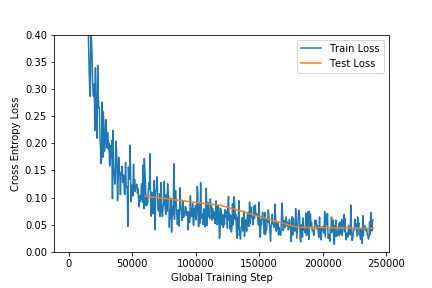
\includegraphics[width=0.7\textwidth]{task2}
\caption{Training loss of 4 epochs}
\label{fig:task2}
\end{figure}
From figure \ref{fig:task2}, we do not see evidence of overfitting with these hyperparameters, as the test loss and final test accuracy corresponds well with the training loss. Had the test loss been significantly worse than the training loss however, one would suspect the network to be overfitted to the training data.

\end{document}

